% $Id: results.tex 1784 2012-04-27 23:29:31Z nicolas.cardozo $
% !TEX root = main.tex

\chapter{Analysis and Results}
\label{cha:results}
This section presents the analysis of theresults of the survey presented in \fref{sec:evaluation}. 
This results are presented according to three sections of the survey: General knowledge (\fref{sec:general-knowledge}),
Task Efectiveness (\fref{sec:tasks-results}) and usability (\fref{sec:usability}). Additionally, a 
discussion section is added analyzing the results form the survey. All aditional data, not mentioned 
on this section, is given in Appendix A.2.

\section{General Knowledge Results}
\label{sec:general-knowledge}
Most of the participants were very experienced on the use of python as it
can be seen in (\fref{fig:general-know} (a)), most of the people had a high level of expertise (over 5)
as they used Python very often in their work and university. 
Most of the people were very familiarized using \ac{RL} algorithms (\fref{fig:general-know} (b)), as they were 
taking a course on the topic. This is very important information, as the bugs required familiarity with \ac{RL} and python 
knowledge to be identified. Furthermore, the students were very familiarized with 
the terminal, this means it would be easy for them to interact with the tool, as the commands 
and the interface require experience using the console (\fref{fig:general-know} (c)). Nevertheless, 
average the 
students weren't familiarized with debuggers, and they only used them very rarely, or used 
Visual Studio Code interface simple features, like breakpoint function. This lead to 
misunderstandings and probably difficulties in making the tasks, as the tool is based on
previous debugger (\fref{fig:general-know} (d)). Also, this made the learning curve of the tool 
steeper than with a person with previous debugger experience.

Note that in the figures in \fref{fig:general-know} the y-axis represents the number of people 
that answered the question with that score, and the x-axis represents score, which could have a 
possible value of 5 being completely agreed, and 1 being completely disagreed.

\begin{figure}
    \centering
    \subfloat[]{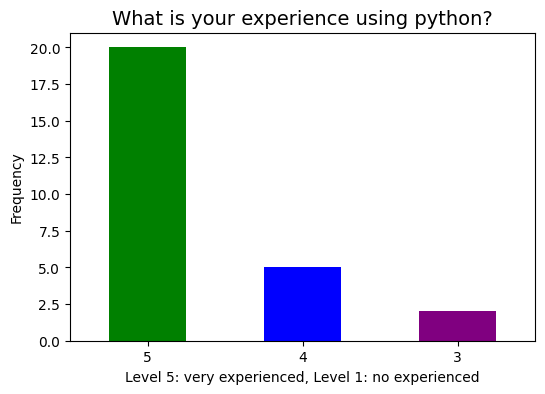
\includegraphics[width=0.25\textwidth]{figures/experience-python.png}} 
    \subfloat[]{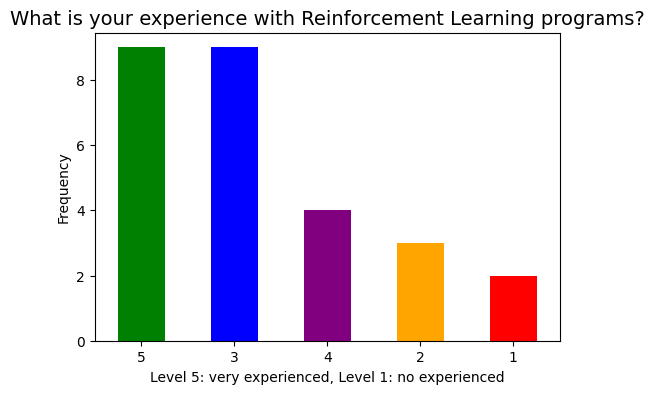
\includegraphics[width=0.25\textwidth]{figures/experience-rl.png}} \\
    \subfloat[]{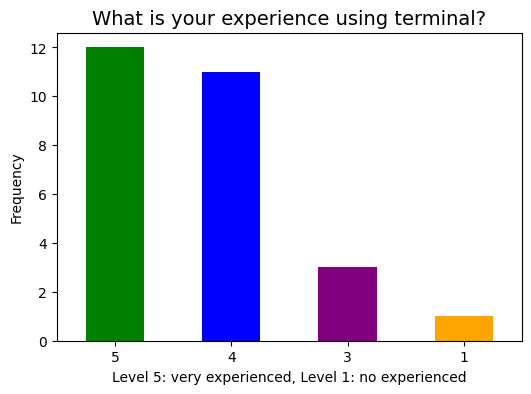
\includegraphics[width=0.25\textwidth]{figures/experience-terminal.png}}
    \subfloat[]{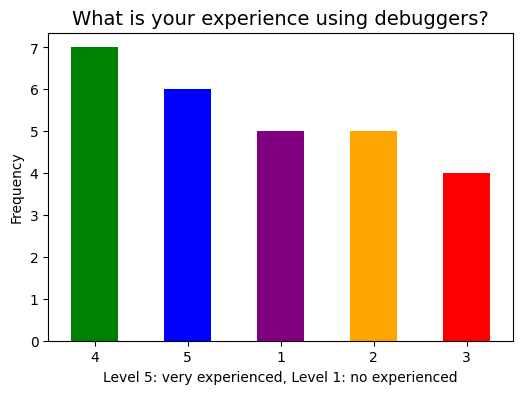
\includegraphics[width=0.25\textwidth]{figures/experience-debuggers.png}}
    \caption{(a) Python Experience (b) RL Experience (c) Terminal Experience (d) Debuggers Experience}
    \label{fig:general-know}
\end{figure}



\section{Tasks Results}
\label{sec:tasks-results}
As there can be seen in the tables \fref{tab:grid-results}, \fref{tab:rooms-results} and 
\fref{tab:cars-results}, most of the people made it through the first task (\fref{fig:task1}),
they thought it was an easy task to solve. This task besides being easy, took them a lot of 
time to complete because this was the task in which they were getting familiarized with the 
tool. The second task was harder than the first one, most of the people took longer to finish the 
task (\fref{fig:task2}), and most of the people had trouble finding the problem to the program. 
This was meant to be as task 2, wasn't meant to be completely wrong, it was just taking huge 
steps, and the error wasn't because a variable definition, but because a changed in the Q-learning
algorithm, which made a lot of students initially confused. Finally, the third task (\fref{fig:task3}) was the hardest 
one, most people had trouble finding the bug. They thought it wasn't an easy task to solve, 
nevertheless, most of the people managed to finish the task in less time than in the other tasks. 
In this case, it is understandable that for the first task besides being 
easy people took longer, because they were getting familiarized with the tool. For the second task,
given the nature of the bug and the fact that the bug was introduced in the Q-learning algorithm, 
it was harder to find the bug, and for that people thought it was harder to solve, but
most of the people finish it. Finally, for the third task, the bug was introduced in the rewards,
people took less as they had more practice with the tool.

Note that in the figures in \fref{fig:general-know} the y-axis represents the number of people 
that answered the question with that score, and the x-axis represents score, which could have a 
possible value of 5 being completely agreed, and 1 being completely disagreed. Except for the 
last question, in which 5 was taking a lot of time, and 1 was taking very little time.

\begin{figure}
    \centering
    \subfloat[]{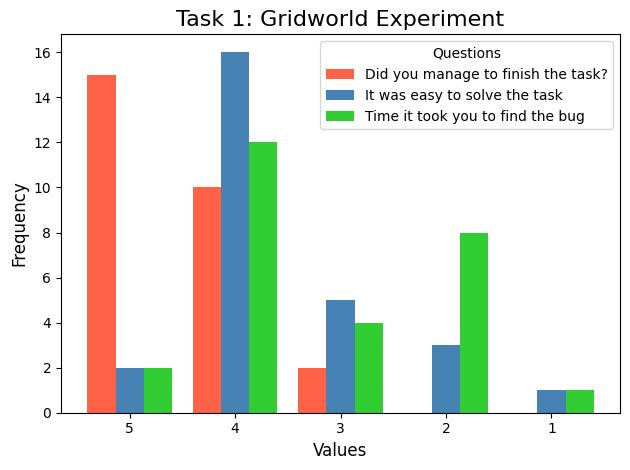
\includegraphics[width=0.25\textwidth]{figures/task1.png}} 
    \subfloat[]{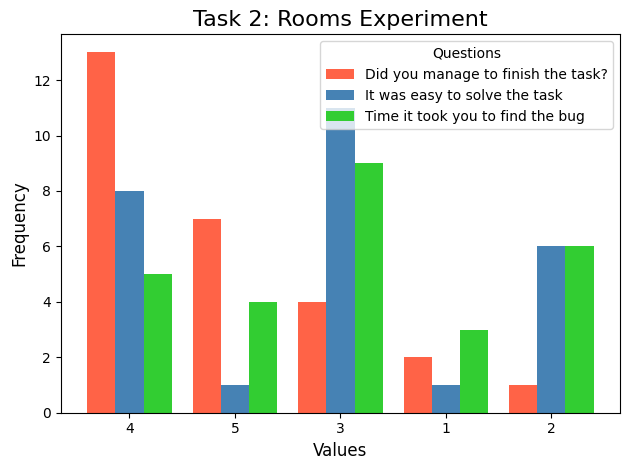
\includegraphics[width=0.25\textwidth]{figures/task2.png}} \\
    \subfloat[]{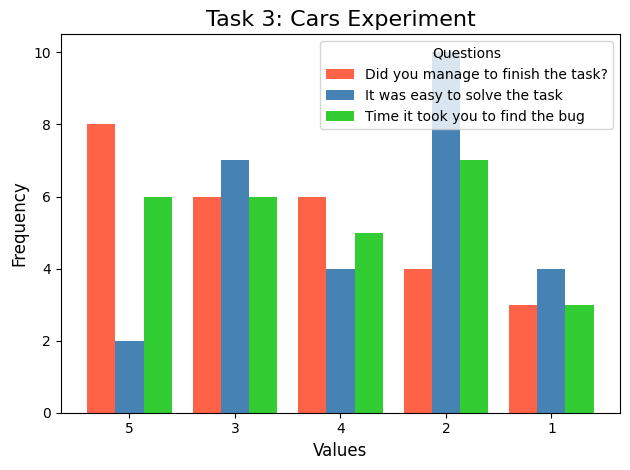
\includegraphics[width=0.25\textwidth]{figures/task3.png}}
    \caption{(a) GridWrold (b) Rooms (c) Driving Assistant}
    \label{fig:general-know}
\end{figure}

\section{Debugger Usability Results}
\label{sec:usability}

Regarding the debugger usability (\fref{tab:general1-debuggers} and \fref{tab:general2-debuggers}), it can 
be seen that the tool was useful,
and the general comments were that the tool would be useful if there was more time to study it. 
And to learn about the tool before using it in real tasks. The 
tool was easy to use, once they got to know it a little better, and they got to practice more with the commands.
Additionally, there were several comments about the tool improving the UI,
as it was hard to understand the tool at first sight, it wasn't similar to the Visual Studio Code 
interface that most of the people were used to use.

Note that in the figures in \fref{fig:general-know} the y-axis represents the number of people 
that answered the question with that score, and the x-axis represents score, which could have a 
possible value of 5 being completely agreed, and 1 being completely disagreed.

\begin{table}[H]
\centering
\resizebox{\columnwidth}{!}{%
\begin{tabular}{
>{\columncolor[HTML]{FFFFFF}}c 
>{\columncolor[HTML]{FFFFFF}}c 
>{\columncolor[HTML]{FFFFFF}}c 
>{\columncolor[HTML]{FFFFFF}}c 
>{\columncolor[HTML]{FFFFFF}}c 
>{\columncolor[HTML]{FFFFFF}}c }
% \multicolumn{6}{c}{\cellcolor[HTML]{FFFFFF}{\color[HTML]{383838} \textbf{Task 2: Rooms Experiment.}}}                                                                                                                                                                                                                                                                                                                                                                                                                                                                                                                                                                                                 \\
{\color[HTML]{383838} \textbf{}}  & {\color[HTML]{383838} \textbf{\begin{tabular}[c]{@{}c@{}}I have found too much \\ inconsistency in this system\end{tabular}}} & {\color[HTML]{383838} \textbf{\begin{tabular}[c]{@{}c@{}}I think most people would learn \\ to use the system quickly\end{tabular}}} & {\color[HTML]{383838} \textbf{\begin{tabular}[c]{@{}c@{}}I found the system quite \\ awkward to use\end{tabular}}} & {\color[HTML]{383838} \textbf{\begin{tabular}[c]{@{}c@{}}I have felt very safe \\ using the system\end{tabular}}} & {\color[HTML]{383838} \textbf{\begin{tabular}[c]{@{}c@{}}I would need to learn a lot \\ of things before I could handle the system\end{tabular}}} \\
{\color[HTML]{383838} \textbf{5}} & {\color[HTML]{383838} 1}                                                                                                      & {\color[HTML]{383838} 7}                                                                                                             & {\color[HTML]{383838} 4}                                                                                           & {\color[HTML]{383838} 7}                                                                                          & {\color[HTML]{383838} 8.0}                                                                                                                        \\
{\color[HTML]{383838} \textbf{4}} & {\color[HTML]{383838} 2}                                                                                                      & {\color[HTML]{383838} 6}                                                                                                             & {\color[HTML]{383838} 7}                                                                                           & {\color[HTML]{383838} 8}                                                                                          & {\color[HTML]{383838} 6.0}                                                                                                                        \\
{\color[HTML]{383838} \textbf{3}} & {\color[HTML]{383838} 4}                                                                                                      & {\color[HTML]{383838} 6}                                                                                                             & {\color[HTML]{383838} 9}                                                                                           & {\color[HTML]{383838} 7}                                                                                          & {\color[HTML]{383838} 4.0}                                                                                                                        \\
{\color[HTML]{383838} \textbf{2}} & {\color[HTML]{383838} 7}                                                                                                      & {\color[HTML]{383838} 6}                                                                                                             & {\color[HTML]{383838} 4}                                                                                           & {\color[HTML]{383838} 4}                                                                                          & {\color[HTML]{383838} 0.0}                                                                                                                        \\
{\color[HTML]{383838} \textbf{1}} & {\color[HTML]{383838} 13}                                                                                                     & {\color[HTML]{383838} 2}                                                                                                             & {\color[HTML]{383838} 3}                                                                                           & {\color[HTML]{383838} 1}                                                                                          & {\color[HTML]{383838} 9.0}                                                                                                                       
\end{tabular}%
}
\caption{General Results Part 1}
\label{tab:general1-debuggers}
\end{table}

\begin{table}[H]
\centering
\resizebox{\columnwidth}{!}{%
\begin{tabular}{
>{\columncolor[HTML]{FFFFFF}}c 
>{\columncolor[HTML]{FFFFFF}}c 
>{\columncolor[HTML]{FFFFFF}}c 
>{\columncolor[HTML]{FFFFFF}}c 
>{\columncolor[HTML]{FFFFFF}}c 
>{\columncolor[HTML]{FFFFFF}}c }
% \multicolumn{6}{c}{\cellcolor[HTML]{FFFFFF}{\color[HTML]{383838} \textbf{Task 2: Rooms Experiment.}}}                                                                                                                                                                                                                                                                                                                                                                                                                                                                                                                                                                                      \\
{\color[HTML]{383838} \textbf{}}  & {\color[HTML]{383838} \textbf{\begin{tabular}[c]{@{}c@{}}I think I would like to use this \\ system frequently\end{tabular}}} & {\color[HTML]{383838} \textbf{\begin{tabular}[c]{@{}c@{}}I find this system \\ unnecessarily complex\end{tabular}}} & {\color[HTML]{383838} \textbf{\begin{tabular}[c]{@{}c@{}}I think the system \\ is easy to use\end{tabular}}} & {\color[HTML]{383838} \textbf{\begin{tabular}[c]{@{}c@{}}I think I would need technical \\ support to use the system\end{tabular}}} & {\color[HTML]{383838} \textbf{\begin{tabular}[c]{@{}c@{}}I find the various functions of the \\ system quite well integrated\end{tabular}}} \\
{\color[HTML]{383838} \textbf{5}} & {\color[HTML]{383838} 7}                                                                                                      & {\color[HTML]{383838} 2}                                                                                            & {\color[HTML]{383838} 5.0}                                                                                   & {\color[HTML]{383838} 9}                                                                                                            & {\color[HTML]{383838} 6}                                                                                                                    \\
{\color[HTML]{383838} \textbf{4}} & {\color[HTML]{383838} 5}                                                                                                      & {\color[HTML]{383838} 7}                                                                                            & {\color[HTML]{383838} 5.0}                                                                                   & {\color[HTML]{383838} 8}                                                                                                            & {\color[HTML]{383838} 13}                                                                                                                   \\
{\color[HTML]{383838} \textbf{3}} & {\color[HTML]{383838} 7}                                                                                                      & {\color[HTML]{383838} 7}                                                                                            & {\color[HTML]{383838} 11.0}                                                                                  & {\color[HTML]{383838} 4}                                                                                                            & {\color[HTML]{383838} 5}                                                                                                                    \\
{\color[HTML]{383838} \textbf{2}} & {\color[HTML]{383838} 7}                                                                                                      & {\color[HTML]{383838} 6}                                                                                            & {\color[HTML]{383838} 6.0}                                                                                   & {\color[HTML]{383838} 3}                                                                                                            & {\color[HTML]{383838} 2}                                                                                                                    \\
{\color[HTML]{383838} \textbf{1}} & {\color[HTML]{383838} 1}                                                                                                      & {\color[HTML]{383838} 5}                                                                                            & {\color[HTML]{383838} 0.0}                                                                                   & {\color[HTML]{383838} 3}                                                                                                            & {\color[HTML]{383838} 1}                                                                                                                   
\end{tabular}%
}
\caption{General Results Part 2}
\label{tab:general2-debuggers}
\end{table}

% \begin{table}[]
% \centering
% \resizebox{\columnwidth}{!}{%
% \begin{tabular}{
% >{\columncolor[HTML]{FFFFFF}}c 
% >{\columncolor[HTML]{FFFFFF}}c 
% >{\columncolor[HTML]{FFFFFF}}c 
% >{\columncolor[HTML]{FFFFFF}}c 
% >{\columncolor[HTML]{FFFFFF}}c 
% >{\columncolor[HTML]{FFFFFF}}c 
% >{\columncolor[HTML]{FFFFFF}}c 
% >{\columncolor[HTML]{FFFFFF}}c 
% >{\columncolor[HTML]{FFFFFF}}c 
% >{\columncolor[HTML]{FFFFFF}}c 
% >{\columncolor[HTML]{FFFFFF}}c }
% \multicolumn{11}{c}{\cellcolor[HTML]{FFFFFF}{\color[HTML]{383838} \textbf{Debugger Usability.}}}                                                                                                                                                                                                                                                                                                                                                                                                                                                                                                                                                                                                                                                                                                                                                                                                                                                                                                                                                                                                                                                                                                                                                                                                                                                         \\
% {\color[HTML]{383838} \textbf{}}  & {\color[HTML]{383838} \textbf{\begin{tabular}[c]{@{}c@{}}I think I would like to use this \\ system frequently\end{tabular}}} & {\color[HTML]{383838} \textbf{\begin{tabular}[c]{@{}c@{}}I find this system \\ unnecessarily complex\end{tabular}}} & {\color[HTML]{383838} \textbf{\begin{tabular}[c]{@{}c@{}}I think the system \\ is easy to use\end{tabular}}} & {\color[HTML]{383838} \textbf{\begin{tabular}[c]{@{}c@{}}I think I would need technical \\ support to use the system\end{tabular}}} & {\color[HTML]{383838} \textbf{\begin{tabular}[c]{@{}c@{}}I find the various functions of the \\ system quite well integrated\end{tabular}}} & {\color[HTML]{383838} \textbf{\begin{tabular}[c]{@{}c@{}}I have found too much \\ inconsistency in this system\end{tabular}}} & {\color[HTML]{383838} \textbf{\begin{tabular}[c]{@{}c@{}}I think most people would learn \\ to use the system quickly\end{tabular}}} & {\color[HTML]{383838} \textbf{\begin{tabular}[c]{@{}c@{}}I found the system quite \\ awkward to use\end{tabular}}} & {\color[HTML]{383838} \textbf{\begin{tabular}[c]{@{}c@{}}I have felt very safe \\ using the system\end{tabular}}} & {\color[HTML]{383838} \textbf{\begin{tabular}[c]{@{}c@{}}I would need to learn a lot \\ of things before I could handle the system\end{tabular}}} \\
% {\color[HTML]{383838} \textbf{5}} & {\color[HTML]{383838} 7}                                                                                                      & {\color[HTML]{383838} 2}                                                                                            & {\color[HTML]{383838} 5.0}                                                                                   & {\color[HTML]{383838} 9}                                                                                                            & {\color[HTML]{383838} 6}                                                                                                                    & {\color[HTML]{383838} 1}                                                                                                      & {\color[HTML]{383838} 7}                                                                                                             & {\color[HTML]{383838} 4}                                                                                           & {\color[HTML]{383838} 7}                                                                                          & {\color[HTML]{383838} 8.0}                                                                                                                        \\
% {\color[HTML]{383838} \textbf{2}} & {\color[HTML]{383838} 7}                                                                                                      & {\color[HTML]{383838} 6}                                                                                            & {\color[HTML]{383838} 6.0}                                                                                   & {\color[HTML]{383838} 3}                                                                                                            & {\color[HTML]{383838} 2}                                                                                                                    & {\color[HTML]{383838} 7}                                                                                                      & {\color[HTML]{383838} 6}                                                                                                             & {\color[HTML]{383838} 4}                                                                                           & {\color[HTML]{383838} 4}                                                                                          & {\color[HTML]{383838} 0.0}                                                                                                                        \\
% {\color[HTML]{383838} \textbf{3}} & {\color[HTML]{383838} 7}                                                                                                      & {\color[HTML]{383838} 7}                                                                                            & {\color[HTML]{383838} 11.0}                                                                                  & {\color[HTML]{383838} 4}                                                                                                            & {\color[HTML]{383838} 5}                                                                                                                    & {\color[HTML]{383838} 4}                                                                                                      & {\color[HTML]{383838} 6}                                                                                                             & {\color[HTML]{383838} 9}                                                                                           & {\color[HTML]{383838} 7}                                                                                          & {\color[HTML]{383838} 4.0}                                                                                                                        \\
% {\color[HTML]{383838} \textbf{4}} & {\color[HTML]{383838} 5}                                                                                                      & {\color[HTML]{383838} 7}                                                                                            & {\color[HTML]{383838} 5.0}                                                                                   & {\color[HTML]{383838} 8}                                                                                                            & {\color[HTML]{383838} 13}                                                                                                                   & {\color[HTML]{383838} 2}                                                                                                      & {\color[HTML]{383838} 6}                                                                                                             & {\color[HTML]{383838} 7}                                                                                           & {\color[HTML]{383838} 8}                                                                                          & {\color[HTML]{383838} 6.0}                                                                                                                        \\
% {\color[HTML]{383838} \textbf{1}} & {\color[HTML]{383838} 1}                                                                                                      & {\color[HTML]{383838} 5}                                                                                            & {\color[HTML]{383838} 0.0}                                                                                   & {\color[HTML]{383838} 3}                                                                                                            & {\color[HTML]{383838} 1}                                                                                                                    & {\color[HTML]{383838} 13}                                                                                                     & {\color[HTML]{383838} 2}                                                                                                             & {\color[HTML]{383838} 3}                                                                                           & {\color[HTML]{383838} 1}                                                                                          & {\color[HTML]{383838} 9.0}                                                                                                                       
% \end{tabular}%
% }
% \end{table}

\section{Discussion}
\label{sec:discussion}

In general, the results of the survey were very positive, most of the people thought that 
the tool was useful specially for the kind of challenges \ac{RL} programs could have. In 
spite of the tool being hard to familiarized with at the beginning, specially for the people who had very 
little experience with debuggers, most of the people thought that the tool was easy to use 
once you get to know it a little better. Additionally, people said that the tool would've 
been useful for the course development, as most of the main errors they had for their homework,
were related to the bugs being introduced in these tasks.

Additionally, it was expected that for the first task people used a bit more time to finish the 
task, besides being an easy task, as they were getting familiarized with the tool. For the second,
task, most of the people had trouble finding the bug, they needed to explore much more within the 
code before finding the bug, compared to the last task. Finally, it was expected that the developers
took less time to find the last bug, as they already had practice with the tool, and they were 
knew how to use it and how to interact with the program. Nevertheless, it was expected that 
the users felt the task harder than the previous one. It was also surprising that for this last task 
they found more bugs than the initially expected one.

\endinput

